\chapter{Types and Expressions}
\label{typeexpr}

In the following sections \emph{Ident} refers to a identifier of the graph model language (see \ref{modelbb}) or the rule set language (see \ref{rulebb}). By analogy \emph{TypeIdent} is a identifier of a type.

\section{Built-In Types}
\label{builtin}
Besides user-defined node types, edge types and enum types, GrGen supports the built-in primitive types in table \ref{builtintypes}.
\begin{table}[htbp]
\begin{tabularx}{\linewidth}{|l|X|}\hline
	\texttt{boolean} & Covers the values \texttt{true} and \texttt{false}. \\
	\texttt{int} & A 32-bit signed integer, in two's complement representation. \\
	\texttt{float}, \texttt{double} & A floating-point number in IEEE 754 format with single precision or double precision respectively. \\
	\texttt{string} & A sequence of digits, letters, underscores and white spaces. Strings are of arbitrary length and may be enclosed by double quotes. If the string contains white spaces, double quotes are mandatory.\\ \hline
\end{tabularx}
\caption{\GrG\ built-in types}
\label{builtintypes}
\end{table}
Table \ref{tabcasts} lists \GrG's implicit type casts and the allowed explicit type casts. Of course you are free to express an implicit type cast by an explicit type cast as well as ``cast'' a type to itself.
\begin{example}
  \texttt{myfloat = myint; mydouble = (float)myint; mystring = (string)mybool} is allowed, \\
  \texttt{myenum = (myenum)int; myfloat = mydouble; myint = (int)mybool} is forbidden.
\end{example}
\begin{table}[htbp]
  \centering
  \begin{tabular}[c]{|c|cccccc|} \hline
    \backslashbox{to}{from} & \texttt{enum} & \texttt{boolean} & \texttt{int} & \texttt{float} & \texttt{double} & \texttt{string}\\ \hline
    \texttt{enum} & --- & & & & & \\ 
    \texttt{boolean} & & --- & & & & \\
    \texttt{int} & \texttt{(int)} & & --- & \texttt{(int)} & \texttt{(int)} & \\
    \texttt{float} & \texttt{(float)} & & implicit & --- & \texttt{(float)} & \\
    \texttt{double} &  \texttt{(double)} & & implicit & implicit & --- & \\
    \texttt{string} &  & \texttt{(string)} & \texttt{(string)} & \texttt{(string)} & \texttt{(string)} & --- \\ \hline
  \end{tabular}
  \caption{\GrG\ type casts.}
  \label{tabcasts}
\end{table}

\section{Expressions}
\label{expressions}
\begin{rail}
  Expression: BoolExpr | IntExpr | FloatExpr | StringExpr | PrimaryExpr ;  
  BoolExpr: ((() | '!') (() | '(' 'boolean' ')') PrimaryExpr) | (BoolExpr '?' BoolExpr ':' BoolExpr) | (BoolExpr BinBoolOperator BoolExpr) | (Expression CompareOperator Expression) | (TypeExpr CompareOperator TypeExpr);
\end{rail}
As in C \cite{isoc}, \texttt{!} negates a Boolean. Table \ref{tabboolops} lists the binary operators for Boolean expressions. The \texttt{?} operator is a simple if-then-else: if the first \emph{BoolExpr} is evaluated to \texttt{true}, the operator returns the second \emph{BoolExpr}, otherwise it returns the third \emph{BoolExpr}.\\
The \emph{CompareOperator} is one of the following operators:
\[ \texttt{<} \;\;\;\;\; \texttt{<=} \;\;\;\;\; \texttt{==} \;\;\;\;\; \texttt{!=} \;\;\;\;\; \texttt{>=} \;\;\;\;\; \texttt{>} \]
Table \ref{compandtypes} describes the semantics of compare operators on type expressions.\\
\begin{table}[htbp]
\label{compandtypes} 
  \centering
  \begin{tabularx}{\linewidth}{|l|X|} \hline
    \texttt{A == B} & True, iff $A$ and $B$ are identical. Different types in a type hierarchy are \emph{not} identical. \\
    \texttt{A != B} & True, iff $A$ and $B$ are not identical. \\
    \texttt{A < B} & True, iff $A$ is a supertype of $B$, but $A$ and $B$ are not identical. \\
    \texttt{A > B} & True, iff $A$ is a subtype of $B$, but $A$ and $B$ are not identical. \\
    \texttt{A <= B} & True, iff $A$ is a supertype of $B$ or $A$ and $B$ are identical. \\
    \texttt{A >= B} & True, iff $A$ is a subtype of $B$ or $A$ and $B$ are identical. \\ \hline
  \end{tabularx}
  \begin{note}
  \texttt{A < B} corresponds to the direction of the arrow in an UML class diagram.
  \end{note}
\caption{Compare operators on type expressions}
\end{table}
The \emph{BinBoolOperator} is one of the operators in table \ref{tabboolops}.
\begin{table}[htbp] 
  \centering
  %\begin{tabularx}{0.45\linewidth}{|ll|} \hline
  \begin{tabular}[c]{|lp{0.6\linewidth}|} \hline
    \begin{tabular}[c]{l} \texttt{\^} \end{tabular} & \begin{tabular}[c]{l} Logical XOR. True, iff either the first or the second \\ Boolean expression is true. \end{tabular} \\ \hline
    \begin{tabular}[c]{l} \texttt{\&\&} \\ \texttt{||} \end{tabular} & \begin{tabular}[c]{l} Logical AND an OR. Lazy evaluation. \end{tabular}\\ \hline
    \begin{tabular}[c]{l} \texttt{\&} \\ \texttt{|} \end{tabular} & \begin{tabular}[c]{l} Logical AND an OR. Complete evaluation. \end{tabular}\\ \hline
  \end{tabular}
  \caption{Binary Boolean operators, in ascending order of precedence}
  \label{tabboolops}
\end{table}

\begin{rail}
  IntExpr: ((() | '+' | '-' | tilde) (() | '(' 'int' ')') PrimaryExpr) | (BoolExpr '?' IntExpr ':' IntExpr) | (IntExpr BinIntOperator IntExpr);
\end{rail}
The $\sim$ operator is a bitwise complement. That means every bit of an integer value will be flipped. The \texttt{?} operator is a simple if-then-else: if the \emph{BoolExpr} is evaluated to \texttt{true}, the operator returns the first \emph{IntExpr}, otherwise it returns the second \emph{IntExpr}.\\ 
The \emph{BinIntOperator} is one of the operators in table \ref{tabbinops}.
\begin{table}[htbp] 
  \centering
  %\begin{tabularx}{0.45\linewidth}{|ll|} \hline
  \begin{tabular}[c]{|lp{0.6\linewidth}|} \hline
    \begin{tabular}[c]{l} \texttt{\^} \\ \texttt{\&} \\ \texttt{|} \end{tabular} & \begin{tabular}[c]{l} Bitwise XOR, AND and OR \end{tabular} \\ \hline
    \begin{tabular}[c]{l} \texttt{\mbox{<}\mbox{<}} \\ \texttt{\mbox{>}\mbox{>}} \\ \texttt{\mbox{>}\mbox{>}\mbox{>}} \end{tabular} & \begin{tabular}[c]{l} Bitwise shift left, bitwise shift right and \\ bitwise shift right preserving the sign \end{tabular}\\ \hline
    \begin{tabular}[c]{l} \texttt{+} \\ \texttt{-} \end{tabular} & \begin{tabular}[c]{l} Addition and subtraction \end{tabular}\\ \hline
    \begin{tabular}[c]{l} \texttt{*} \\ \texttt{/} \\ \texttt{\%} \end{tabular} & \begin{tabular}[c]{l}Multiplication, integer division and modulo \end{tabular} \\ \hline
  \end{tabular}
  \caption{Binary integer operators, in ascending order of precedence}
  \label{tabbinops}
\end{table}

\begin{rail}  
  FloatExpr: ((() | '+' | '-') (() | '(' ('float' | 'double') ')') PrimaryExpr) | (BoolExpr '?' FloatExpr ':' FloatExpr) | (FloatExpr ('+' | '-' | '*' | '/') FloatExpr);
\end{rail} 
The \texttt{?} operator is a simple if-then-else: if the \emph{BoolExpr} is evaluated to \texttt{true}, the operator returns the first \emph{FloatExpr}, otherwise it returns the second \emph{FloatExpr}.

\begin{rail}
  StringExpr: PrimaryExpr | StringExpr '+' StringExpr;
\end{rail}
The operator \texttt{+} concatenates two strings.

\begin{rail} 
  PrimaryExpr: '(' Expression ')' | Ident (() | '.' Ident) | (EnumType '::' Ident) | Constant;
  Constant: Number | HexNumber | QuotedText | 'true' | 'false';
\end{rail}
\begin{description}
  \item[Number.] Is an \texttt{int}, \texttt{float} or \texttt{double} constant in decimal notation.
  \item[HexNumber.] Is an \texttt{int} constant in hexadecimal notation starting with \texttt{0x}.
  \item[QuotedText.] Is a string constant. A sequence of characters, enclosed by double quotes.
\end{description} 

\section{Type Related Conditions}
\label{typeexpressions}

\begin{rail}
  TypeExpr: TypeIdent | 'typeof' '(' Ident ')' ;
\end{rail}
A type expression identifies a type (and -- in terms of matching -- also its subtypes). A type expression is either a type identifier itself or the type of a graph element. So \emph{Ident} has to be a node or edge identifier.
\begin{example}
The following rule will add a reverse edge to an one-way street.
\begin{grgen}
rule oneway {
    pattern{
        a:Node -x:street-> y:Node;
        negative{
            y -:typeof(x)-> a;
        }
    } 
    replace{
      a -x-> y;
      y -:typeof(x)-> a;
    }
}
\end{grgen}
Remember that we have several subtypes of \texttt{street}. By the aid of the \texttt{typeof} operator, the reverse edge will be automatically typed correctly (the same type as the one-way edge). This behavior is not possible without the \texttt{typeof} operator.
\end{example}

\begin{rail}
  TypeConstraint: backslash '(' (TypeExpr + '+')  ')' ; 
\end{rail}
A type constraint is used to exclude parts of the type hierarchy. The operator \texttt{+} is used to identify a union of types.
\begin{example}
\begin{tabularx}{\linewidth}{c|X}
  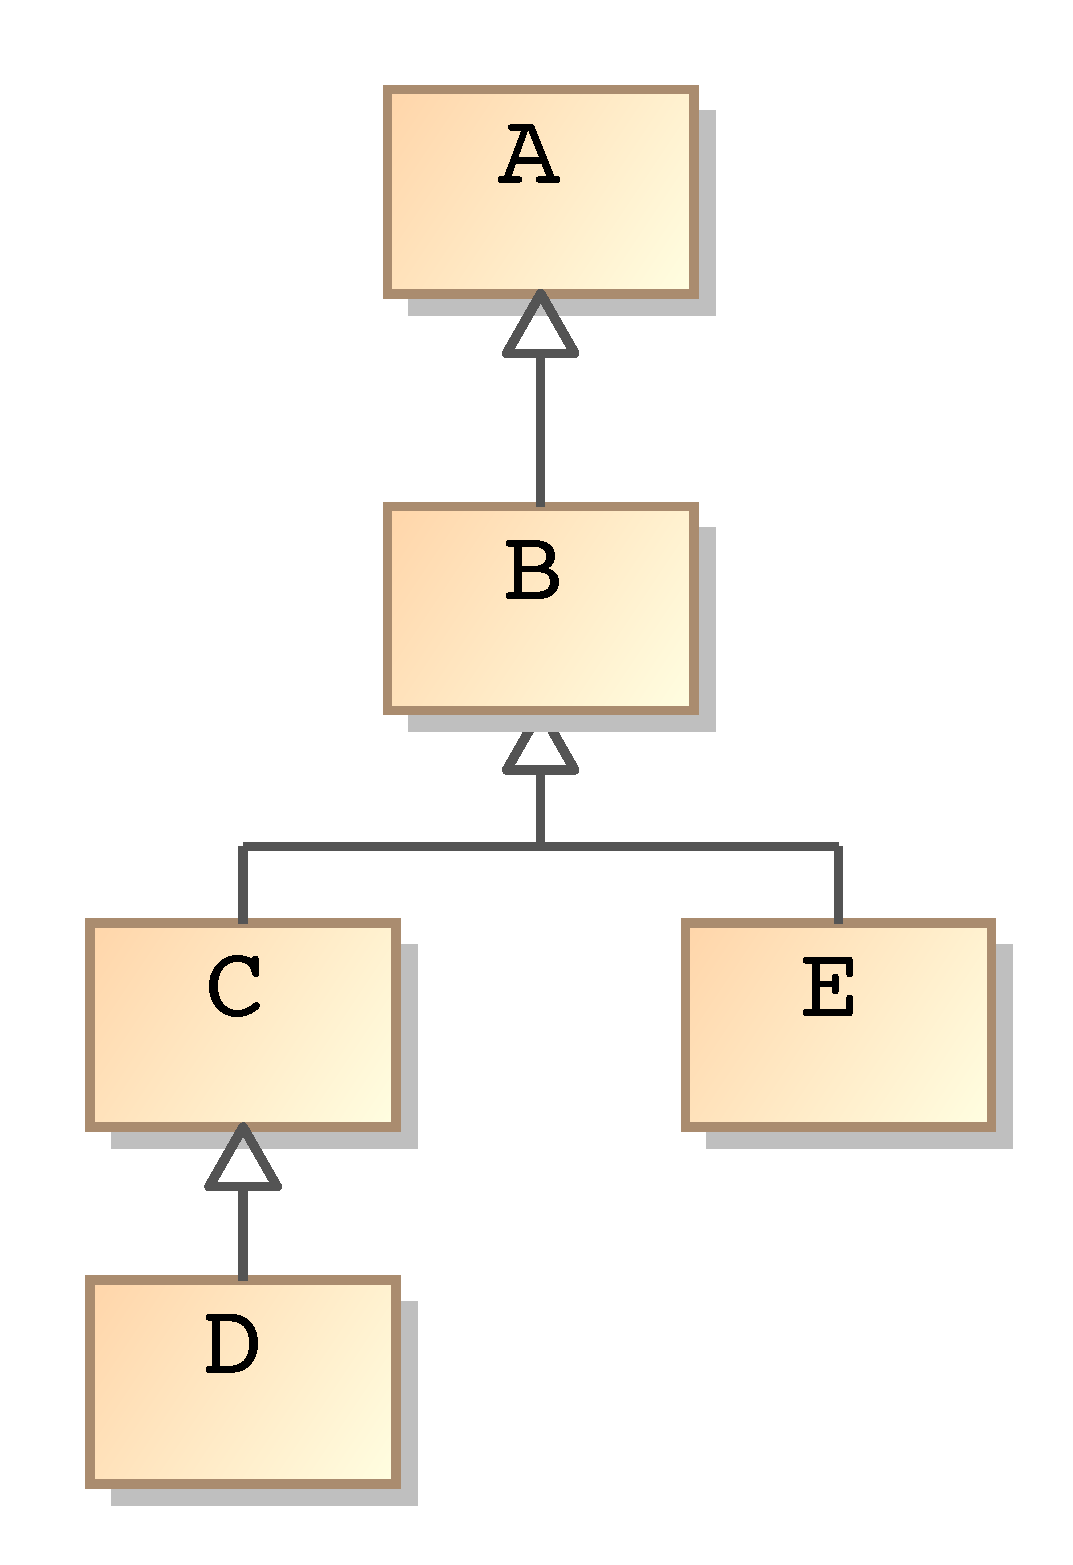
\includegraphics[width=0.25\linewidth]{fig/hierarchy}
  The expression \texttt{A\char"5C (C+E)} applied to the type hierarchy on the left site covers $A$ and $B$.
\end{tabularx}
\end{example}

\section{Annotations}
\label{annotations}

Identifier definitions can be annotated by pragmas. Annotations are key-value pairs.
\begin{rail}
  IdentDecl: Ident (() | '[' (Ident '=' Constant + ',') ']');
\end{rail}
Although you can use any key-value pairs between the brackets, only the identifier \texttt{prio} has an effect so far.
\begin{table}[htbp]
\begin{tabularx}{\linewidth}{|lllX|} \hline
  \textbf{Key} & \textbf{Value Type} & \textbf{Applies to} & \textbf{Meaning} \\ \hline
  \texttt{prio} & int & node, edge & Changes the ranking of a graph element for search plans. The default is \texttt{prio}=1000. Graph elements with high values are likely to appear prior to graph elements with low values in search plans. {\small \textbf{Example:} We search the pattern \texttt{v:NodeTypeA -e:EdgeType-> w:NodeTypeB}. We have a host graph with about 100 nodes of \texttt{NodeTypeA}, 1,000 nodes of \texttt{NodeTypeB} and 10,000 edges of \texttt{EdgeType}. Furthermore we know that between each pair of \texttt{NodeTypeA} and \texttt{NodeTypeB} there exists at most one edge of \texttt{EdgeType}. \GrG\ can use this information to improve the initial search plan, if we adjust the pattern like \texttt{v[prio=10000]:NodeTypeA -e[prio=5000]:EdgeType-> w:NodeTypeB}}. \\ \hline
\end{tabularx}
\caption{Annotations}
\label{tabannotations}
\end{table}



